\documentclass[a4paper, 12pt]{article}
\usepackage{titling}
\usepackage{array}
\usepackage{booktabs}
\usepackage{graphicx}
\usepackage{subcaption}
\usepackage{amsmath}
\setlength{\heavyrulewidth}{1.5pt}
\setlength{\abovetopsep}{4pt}

\setlength{\droptitle}{-7em}

\title{Scientific Experimentation and Evaluation \\
	- Homework 1 -}
\author{Bach Ha, Minh Nguyen}
\date{Lecture date: 27 September 2016}

\begin{document}
	
	\maketitle
	
	
	\begin{enumerate}
		\item \textbf{Experiment}
		\begin{itemize}
			\item Perform 5 experiments, in which a robot move with different translational and angular velocities setting:
				\begin{itemize}
					\item Move straight
					\item Move in an slight arc to left
					\item Move in an slight arc to right
					\item Move in an large arc to left
					\item Move in an large arc to right
				\end{itemize}
			\item Each experiment is repeated 20 times.
			\item End pose of the robot is recorded.
		\end{itemize}
		
		\item \textbf{Bill of material (BOM)}
		\begin{itemize}
			\item 1x LEGO NxT robot
			\item 1x White A0 paper sheet
			\item 1x Pencil
			\item 1x Ruler  200 mm
			\item 1x Ruler 1000 mm
		\end{itemize}
		
		\begin{figure}
		\centering
		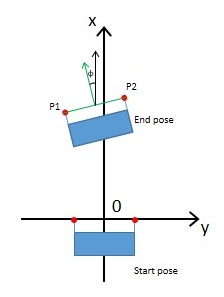
\includegraphics[width=0.5\linewidth]{Img/Img1}
		\caption{Experiment setup}
		\label{fig:img1}
		\end{figure}
		
		\begin{figure}
			\centering
			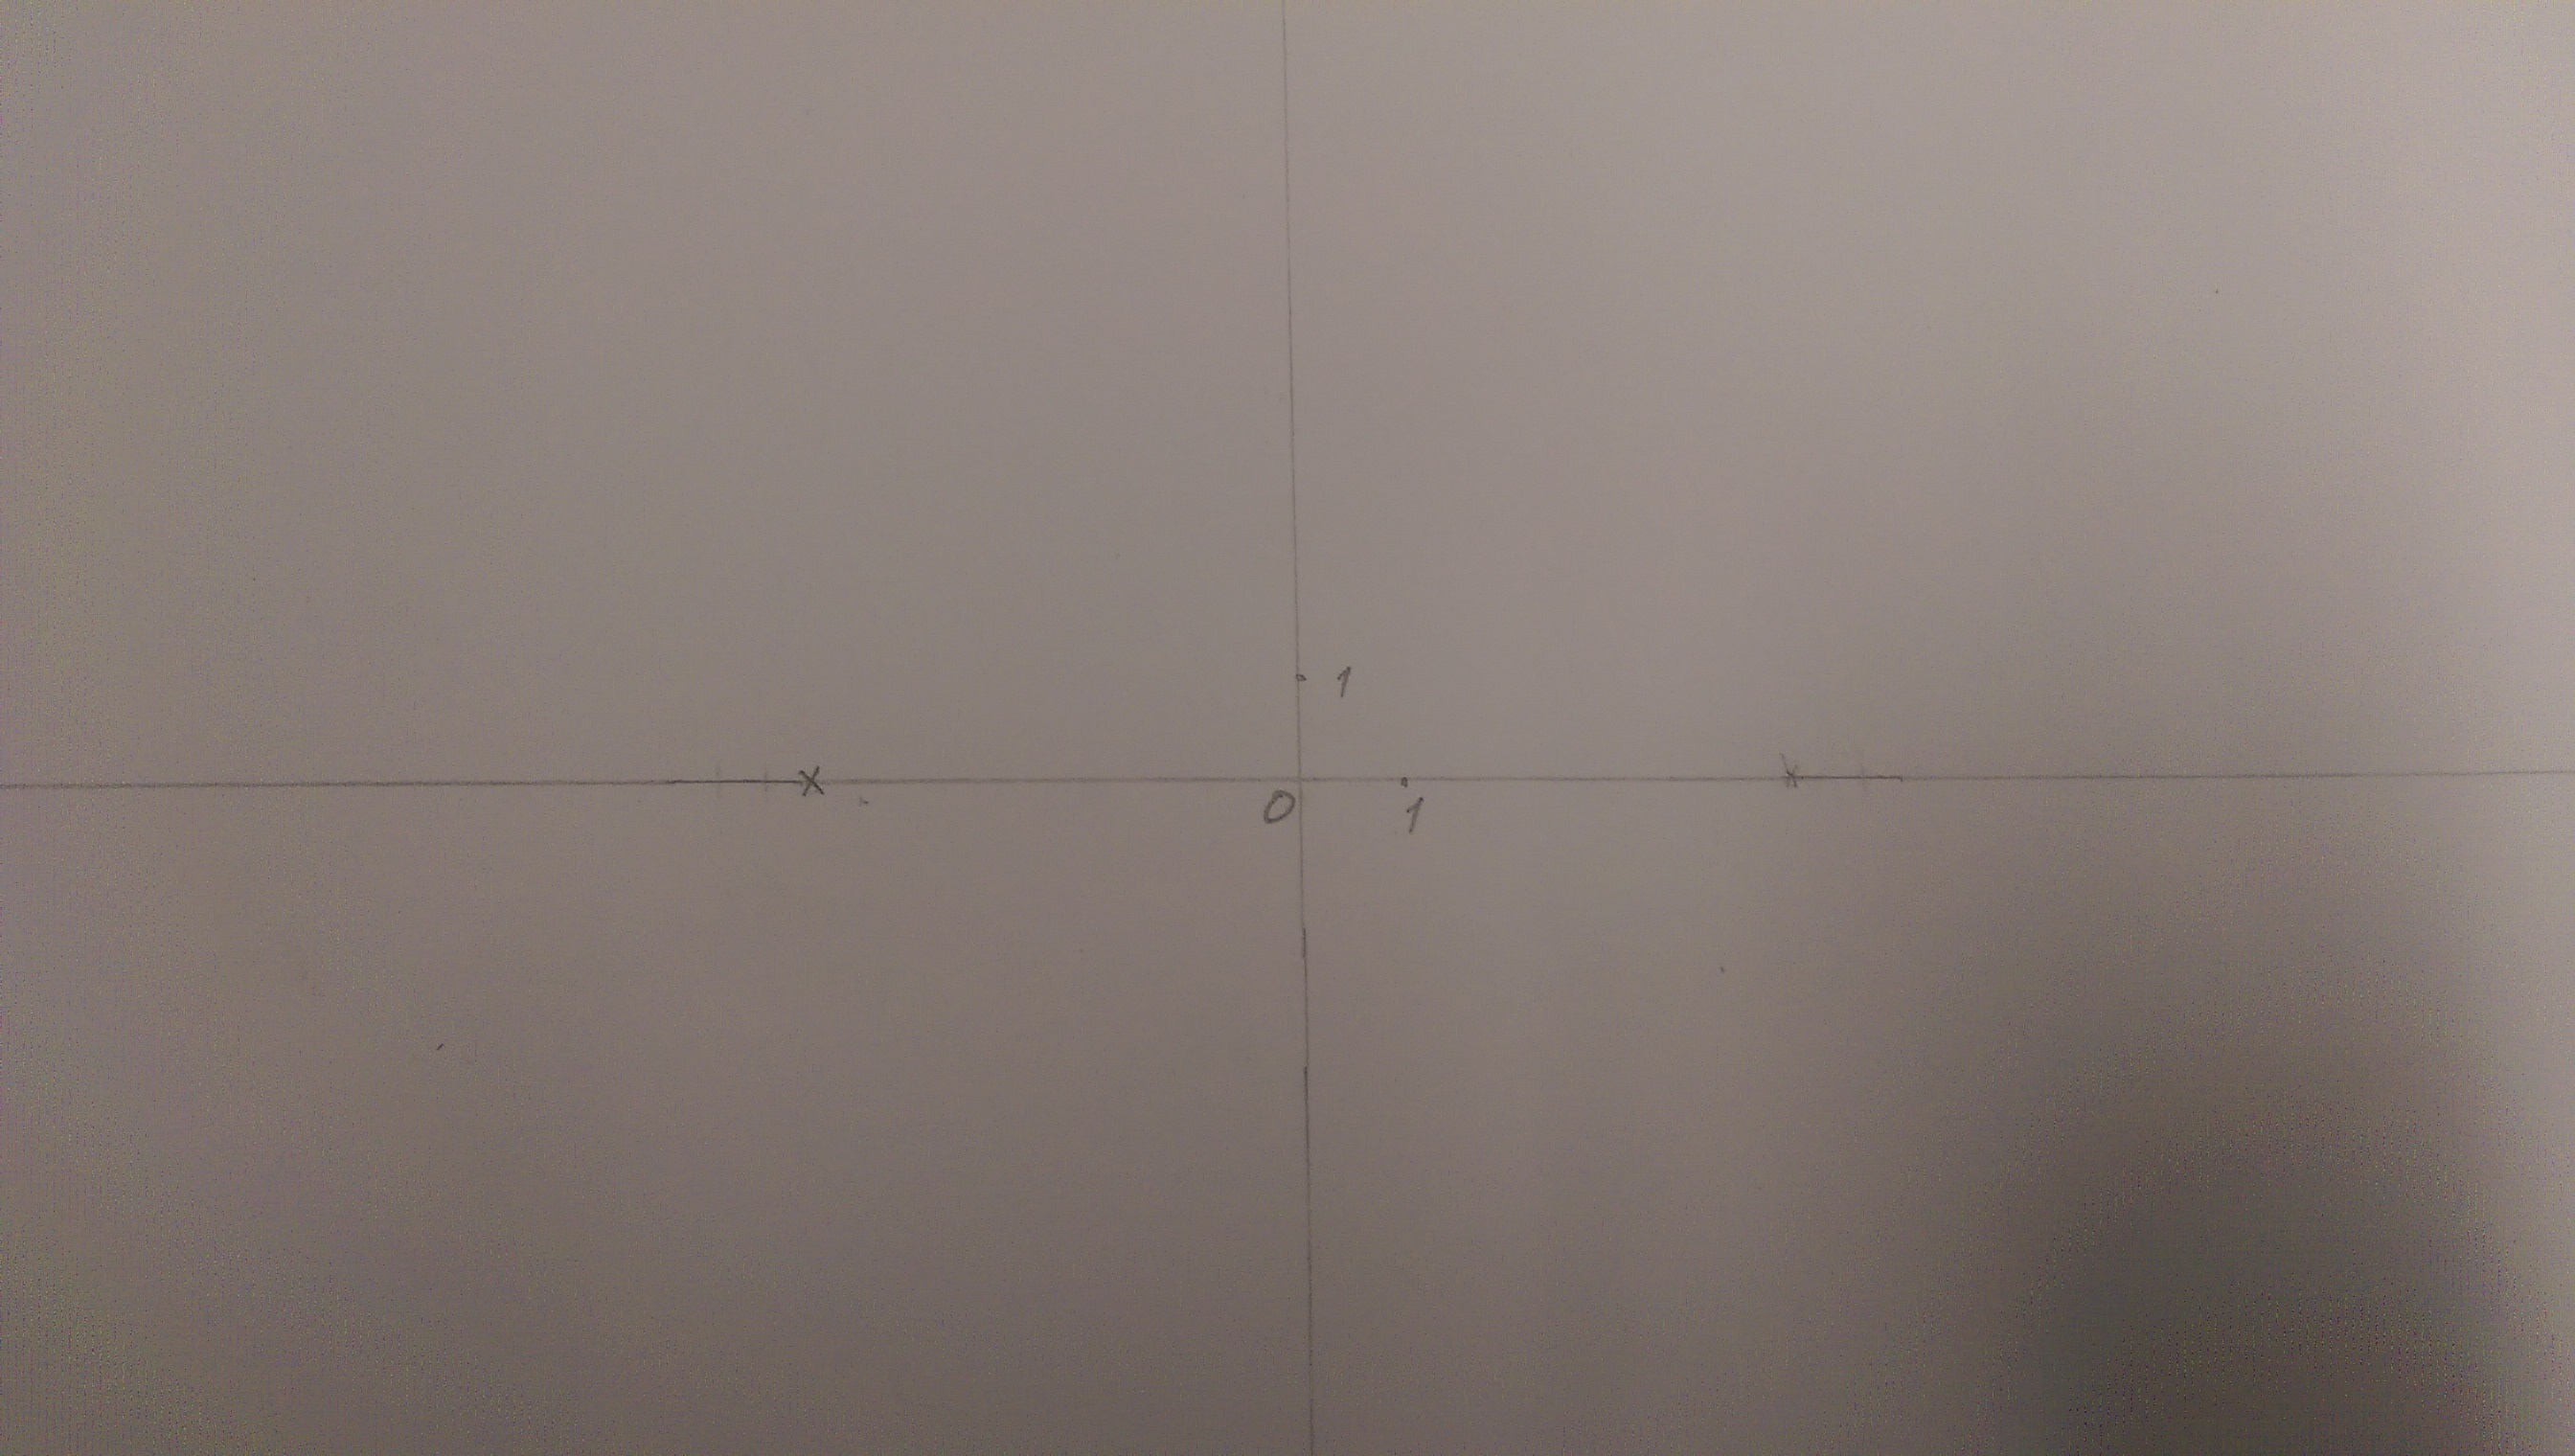
\includegraphics[width=1\linewidth]{Img/IMAG0144}
			\caption{Starting point}
			\label{fig:img2}
		\end{figure}
		
		\begin{figure}[!tbp]
			\centering
			\begin{minipage}[b]{1\textwidth}
				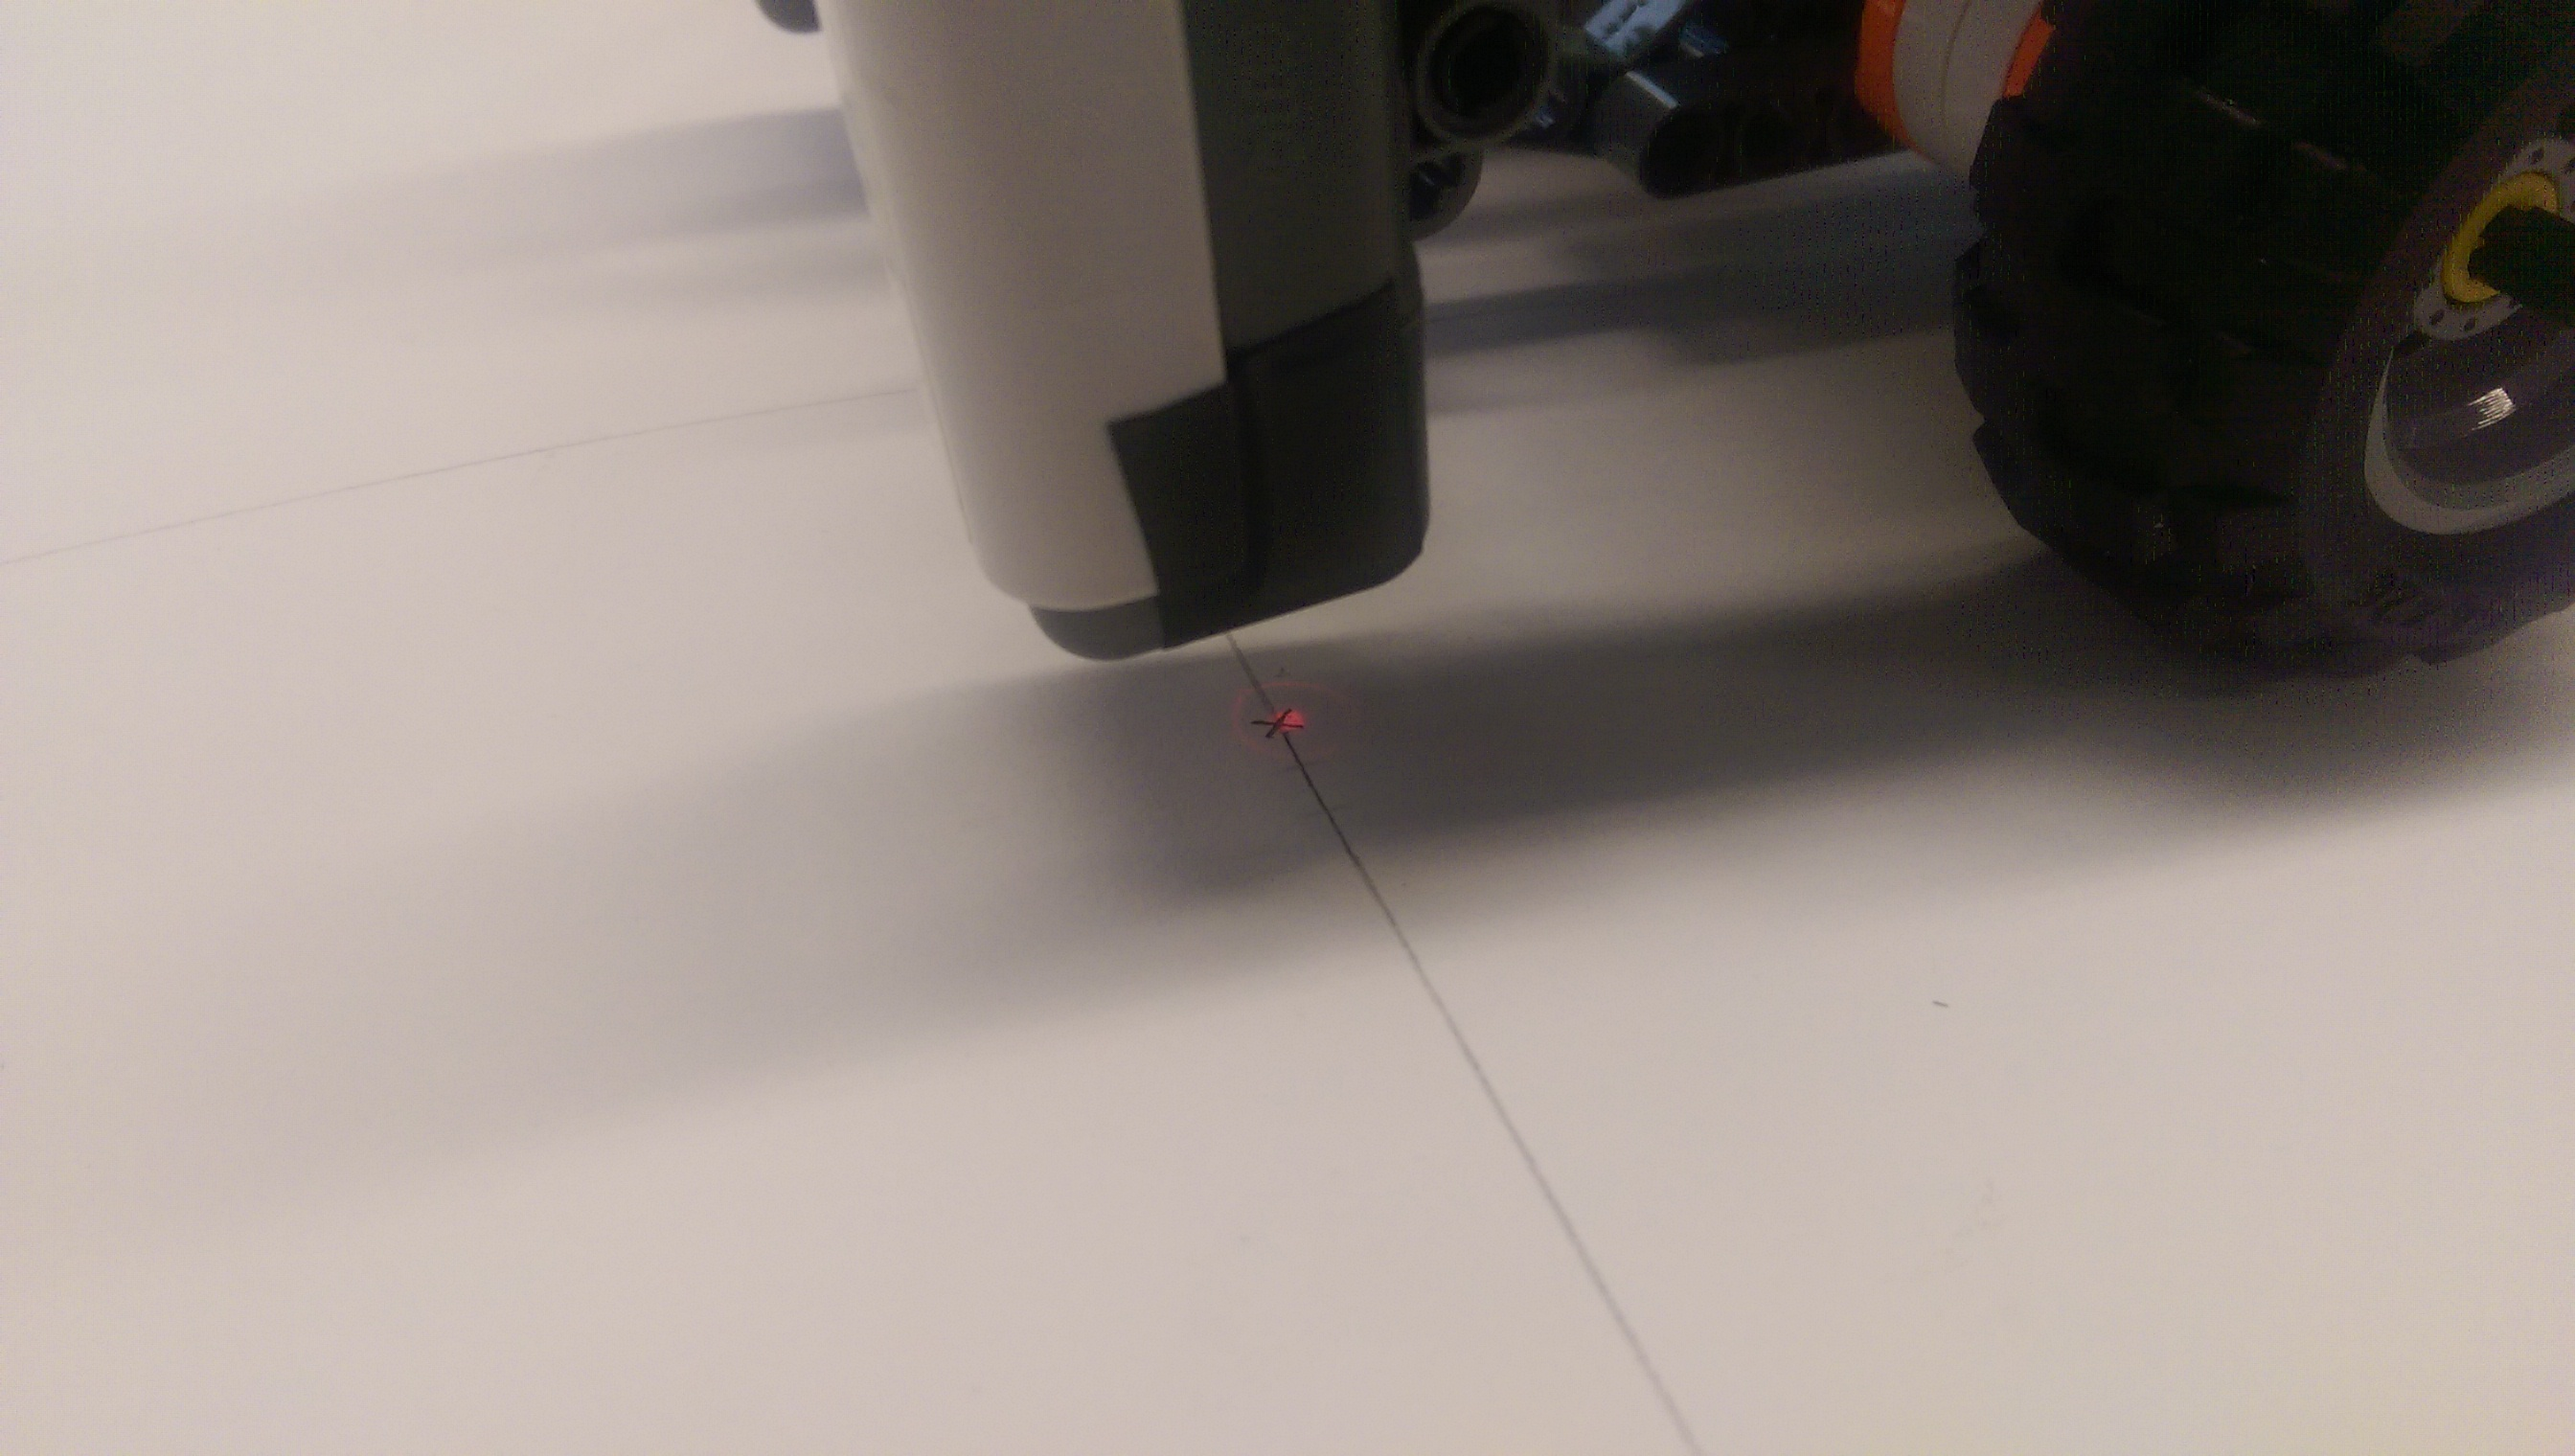
\includegraphics[width=1\linewidth]{Img/IMAG0142}
				\caption{Left marker}
				\label{fig:img3}
			\end{minipage}
			\hfill
			\begin{minipage}[b]{1\textwidth}
				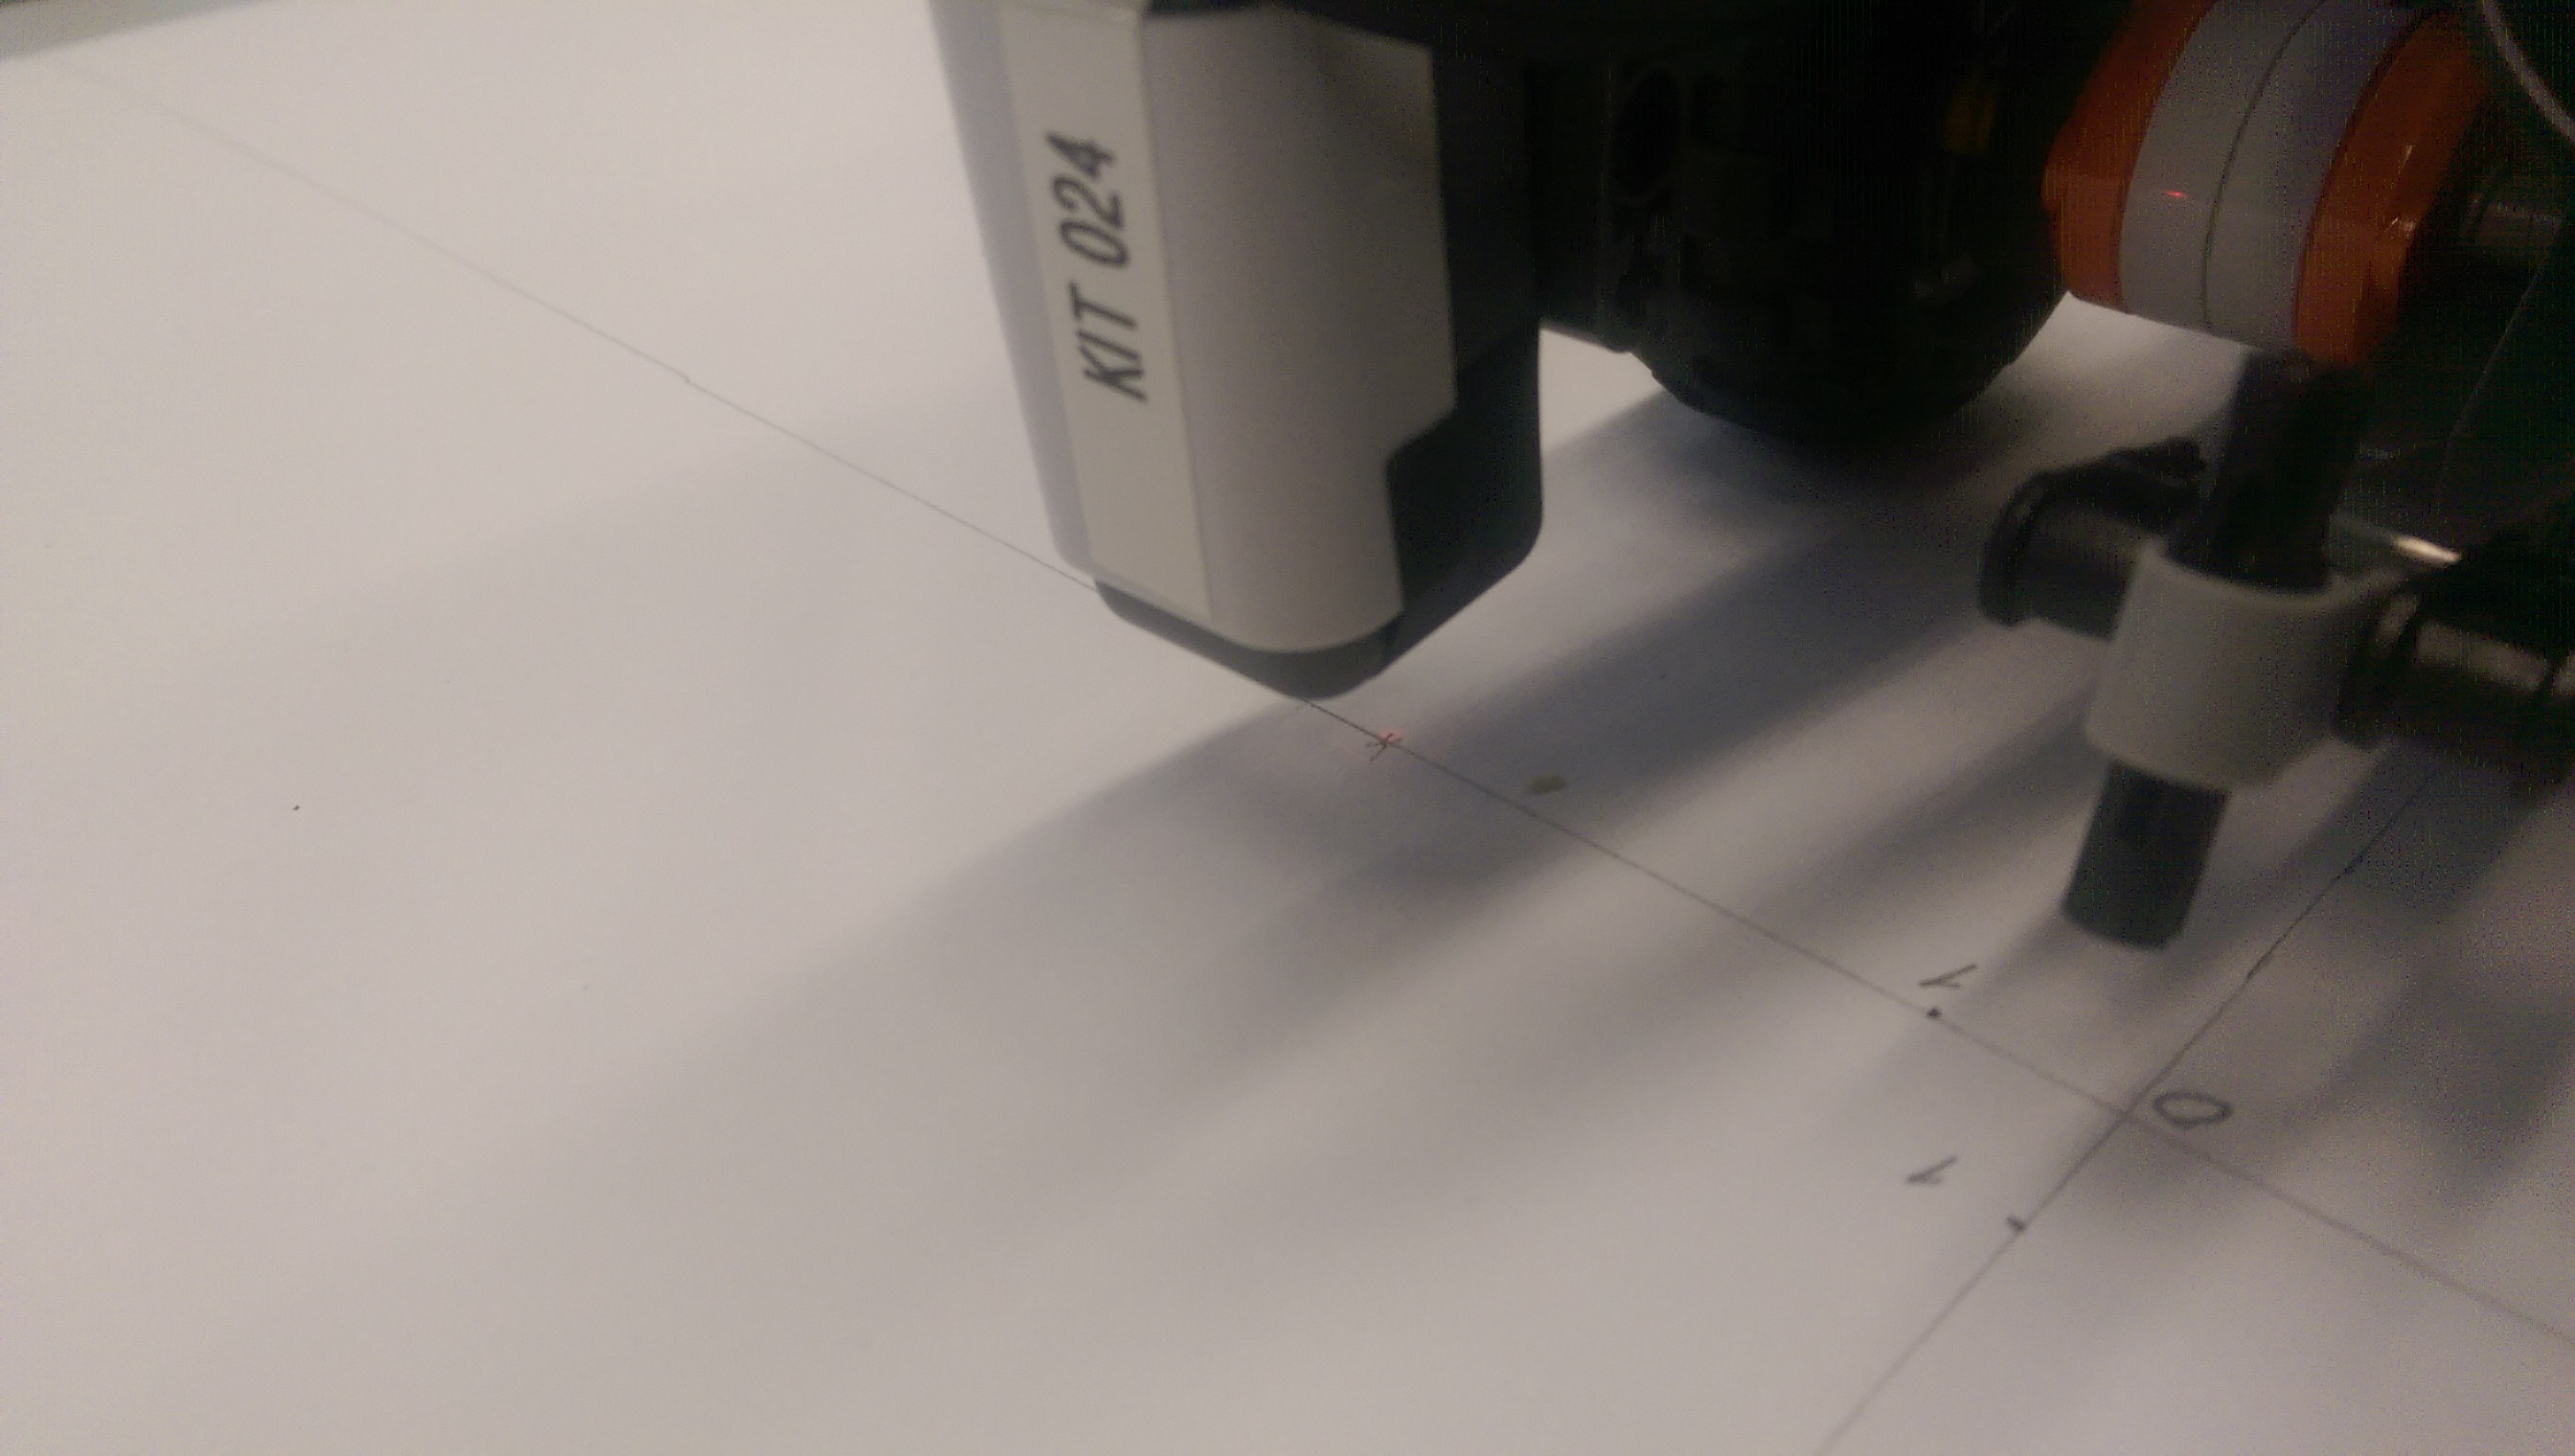
\includegraphics[width=1\linewidth]{Img/IMAG0141}
				\caption{Right marker}
				\label{fig:img4}
			\end{minipage}
		\end{figure}
		
		\item \textbf{Experiment design:}
		\begin{itemize}
			\item Measurand: linear and angular displacement
			\item Measurement facility: ruler, white sheet of paper for marking poses and locations.
			\item DUT: Nxt robot assembled as instructed
			\item Measuring principle: linear comparison
			\item Experiment method:
				\begin{itemize}
					\item Robot is equipped with two red lights pointing down to the paper.
					\item These lights are used to mark two point P1, and P2, which can be used to calculate robot's pose.
					\item Robot always start at the same position with pose (0,0,0).
					\item After the experiment, x-y coordinate of P1, and P2 at the end position are recorded.
					\item Robot's pose is calculated from P1, P2 using the following equation:
					\begin{align*}
						\phi &= \arccos(\dfrac{y_2 - y_1}{\sqrt{(y_2 - y_1)^2 + (x_2 - x_1)^2}}) \\
						x &= \dfrac{x_1 + x_2}{2} - d\cos(\phi)  \\
						y &= \dfrac{y_1 + y_2}{2} + d\sin(\phi) \\
					\end{align*}
						d is the distance from $P_1P_2$'s middle point to the robot center.		
								
				\end{itemize}
			
		\end{itemize}
		
		\item \textbf{Potential error sources:}
		\begin{itemize}
			\item The robot and measurement equipment:
			\begin{itemize}
				\item Structure of robot and marker placement.
				\item Loose connection between parts of the robot.
				\item Power different between two motors.
				\item Different start time of two motors.
				\item Change of battery level during experiment.
				\item Different in friction of each wheel and surface.
				\item Non-uniform friction on the paper sheet.
				\item Ruler's imprecision.
			\end{itemize}
			\item Error in placing the robot at starting position.
			\item Error in marking end position.
			\item Drawing of measuring lines.
			\item Reading of measurement from the paper sheet
			\item Rounding error in pose calculation.
		\end{itemize}
		
	\end{enumerate}
	
	
	
\end{document}
